%%%%%%%%%%%%%%%%%%%% author.tex %%%%%%%%%%%%%%%%%%%%%%%%%%%%%%%%%%%
%
% sample root file for your "contribution" to a contributed volume
%
% Use this file as a template for your own input.
%
%%%%%%%%%%%%%%%% Springer %%%%%%%%%%%%%%%%%%%%%%%%%%%%%%%%%%


% RECOMMENDED %%%%%%%%%%%%%%%%%%%%%%%%%%%%%%%%%%%%%%%%%%%%%%%%%%%
\documentclass[graybox]{svmult}
\usepackage[a4paper]{geometry}

% choose options for [] as required from the list
% in the Reference Guide

\usepackage{mathptmx}       % selects Times Roman as basic font
\usepackage{helvet}         % selects Helvetica as sans-serif font
\usepackage{courier}        % selects Courier as typewriter font
\usepackage{type1cm}        % activate if the above 3 fonts are
                            % not available on your system
%
\usepackage{makeidx}         % allows index generation
\usepackage{graphicx}        % standard LaTeX graphics tool
                             % when including figure files
\usepackage{multicol}        % used for the two-column index
\usepackage[bottom]{footmisc}% places footnotes at page bottom

%
\usepackage{url}
\usepackage{amssymb}

% see the list of further useful packages
% in the Reference Guide

\makeindex             % used for the subject index
                       % please use the style svind.ist with
                       % your makeindex program

%%%%%%%%%%%%%%%%%%%%%%%%%%%%%%%%%%%%%%%%%%%%%%%%%%%%%%%%%%%%%%%%%%%%%%%%%%%%%%%%%%%%%%%%%

\begin{document}

\title*{Performance Evaluation Experiments of Bitcoin SV Scaling Test Network}
% Use \titlerunning{Short Title} for an abbreviated version of
% your contribution title if the original one is too long
\author{Akihiro Fujihara and Takaaki Yanagihara}
% Use \authorrunning{Short Title} for an abbreviated version of
% your contribution title if the original one is too long
\institute{Akihiro Fujihara \at Chiba Institute of Technology, 2-17-1 Tsudanuma, Narashino, Chiba 275-0016, JAPAN, \email{akihiro.fujihara@p.chibakoudai.jp}
\and Takaaki Yanagihara \at Chiba Institute of Technology, 2-17-1 Tsudanuma, Narashino, Chiba 275-0016, JAPAN, \email{s1522313qq@s.chibakoudai.jp}}
%
% Use the package "url.sty" to avoid
% problems with special characters
% used in your e-mail or web address
%
\maketitle

\abstract{
Bitcoin SV Scaling Test Network (STN) is an experimental network for testing Bitcoin scalability using on-chain technology. 
A large amount of transactions are always sent to the peer-to-peer network, and huge blocks are constantly generated. 
In this study, by running our STN node, occupancy rate of transaction processing and blockchain split probability are estimated. 
As a result, the estimated occupancy rate was about 1.04 and the estimated split probability was 8.5\%.
In addition, transaction processing performance was experimentally evaluated by sending transactions including OP\_RETURN script as frequently as once per minute during one week. 
As a result, the estimated probability that a transaction was finally approved was 98\%.
We also confirmed that the distribution of latency time until a transaction is approved follows a power-law distribution at the high tail.
From these results, we concluded that it is consistent to analyze STN using the theory of priority queueing. 
}


\section{Introduction}
\label{sec:intro}
The origin of the word ``BlockChain'' (Hereinafter abbreviated as BC) is a theoretical study on distributed timestamp services for electronic documents by Haber and Stornetta in the early 1990s
\cite{HS1991,BHS1993,HS1997}.
At that time, the Internet was insufficiently developed, and it was difficult to make the proposed services in a real network environment.
However, the environment had been prepared by the time that Bitcoin \cite{nakamoto} appeared in 2008, and the operation of the peer-to-peer (P2P) electronic cash system started on January 3, 2009.
Since then, the system has never been down until today. 
By this achievement by Bitcoin, BC has attracted attention even though it is essentially the same technology as the distributed time stamp services.
The innovative new idea proposed in Bitcoin was not BC, but Nakamoto Consensus (仲基合意), where an unspecified number of nodes participating in the P2P network form a consensus on BC. 
Although studies on consensus algorithms in distributed systems had been conducted before the advent of Bitcoin, Nakamoto Consensus was innovative in the sense that it proposed a method to form consensus among unspecified number of nodes on the Internet scale by combining multiple mechanisms such as Proof of Work (PoW)\cite{DN1993,JJ1999}, longest-chain rule, and incentive mechanism.


A core application of Bitcoin is micropayment where transactions of less than one yen or cent that can be realized by making transaction fees extremely low. 
Micropayment makes it possible to collect near zero or the level at which people don't care about paying charges from a large number of users when using various services on the Internet. 
Therefore, Bitcoin has the potential to create new decentralized economic mechanisms that have never existed before.
However, the current Bitcoin Core (BTC) \cite{btc} is not used for ordinary payments as an electronic cash system, but has become a store-of-value system for speculative purposes. 
Behind this, there is a technical problem that make BTC practically difficult to perform many micropayments. 


Since the block size limit of BTC is 1 MB, blocks larger than 1 MB are rejected by miners. 
Also, the average block generation time interval for BTC is controlled to ten minutes by a difficulty adjustment algorithm. 
This means that transaction processing capacity is about 7 Transactions Per Second (TPS) at maximum, which is much slower than 56,000 TPS of VISA credit cards. 
To speed up the transaction processing capacity, one might think to simply increase the block size limit or shorten the average block generation time interval. 
However, the larger the block size is, the more time it takes to transfer and share the block to all nodes on the P2P network. 
Therefore, another block is easily generated before the previously generated block is fully distributed to the whole P2P network, and BC split probability increases in general. 
When BC splits, the hash rate that drives block generation is fragmented and the system security is degraded. 
The same problem occurs even if the average block generation time interval is shorter than ten minutes. 
For these reasons, there are technical difficulties in improving the transaction processing capacity, which is called BC scalability problem.


Various research proposals have been made to solve the scalability problem \cite{ZHZB2020} and we are also engaged in this problem with some previous works \cite{Fujihara2018,Fujihara2019,Fujihara2020,YF2021a,YF2021b}.
On the other hand, Lightning network \cite{PD2016}, in which a large amount of transactions are executed outside BC, and only the final transaction output is recorded on BC at once, is attracting attention to reduce the amount of approved transactions. 
This is called off-chain scaling technique and it avoids the scalability problem by using a mechanism outside BC. 
Off-chain technology seems good, but individual transaction processing are not recorded on BC.


Unfortunately, Bitcoin has a history of being used as an illegal transaction platform in darknet markets.
In recent years, however, many cases have been reported that managers and users of these markets have been arrested \cite{silkroad,alphabay,welcome2video}.
These arrests are based on the fact that transactions published on the BC are tamper resistant and are used as legal evidence.
From this point of view, if the off-chain scaling technology spreads, the number of transactions that cannot be tracked and audited increases, making it difficult to control illegal transactions in the darknet market and becoming a hotbed for money laundering or terrorist financing. 
For this reason, considering the balance with law and ethics, it is ultimately required to solve the scalability problem by on-chain scaling technology to record all transactions on BC. 


To do this, BloXroute\cite{bloX} introduced the network layer called Blockchain Distribution Network for additionally connecting to the P2P network to propagate larger blocks in a shorter time. 
The effort to increase the block size limit is being experimented by a test network of Bitcoin SV (BSV) \cite{bsv} called Scaling Test Network (STN) \cite{bitcoinscaling}.
The block size limit of BSV is eliminated, and 
as of May 31, 2022, the average transaction processing capacity of last 24 hours was reportedly 1,809 TPS, and the largest block size ever mined was 4 GB. 


This paper reports our experimental results of data analysis and performance evaluation of transaction processing in STN. 
The contribution of this paper is summarized below: 
%
\begin{itemize}
  \item Using the queueing theory, we investigate the time variation of occupancy rate on transaction processing. 
	We show that the estimated occupancy rate exceeded one during most of the time. 
\item Using the command \textit{bitcoin-cli}, we estimate the BC split probability. 
	We show that the split probability for BTC is theoretically calculated as 2\%, while that for BSV STN is experimentally estimated as about 8.5\%.
	Using this result, the average block propagation time for BSV STN is estimated as about 53 seconds. 
  \item We also experimentally measured the latency time until transactions containing data with OP\_RETURN script is approved by sending transactions as frequent as once per minute during one week. 
	As a result, the probability that a transaction is finally approved is 98\%, and the latency time distribution tends to follow a power-law distribution with its exponent 3/2, which is consistent with the theory of priority queueing. 
\end{itemize}
%




\section{Related Works}
\label{sec:rworks}

\subsection{Calculation of Blockchain Split Probability}
\label{sec:fork}

It is known that the block generation time interval of Bitcoin follows an exponential distribution. 
%
\begin{equation}
	F(t) = P(T \le t) = \int_{0}^{t} \lambda e^{-\lambda t'} dt' = 1 - e^{-\lambda t}, \label{eq:exp}
\end{equation}
where the parameter $\lambda$ is the inverse of the average block generation time interval.
For Bitcoin, the interval is $1 / \lambda = 10$ minutes $= 600$ seconds.


The average latency time for a block to spread to 90\% of all the nodes in the P2P network of BTC is experimentally measured as $t = \tau_{fork} \fallingdotseq 12$ seconds in 2015 before Compact Block Relay is applied \cite{bloX}. 
If another block is generated before the block is spread over the whole network, BC splits. 
Therefore, the BC split probability of BTC can be calculated as 2\% by the following calculation. 
%
\begin{equation}
  F(\tau_{fork}) = P(T \le \tau_{fork}) = 1 - e^{-\lambda \tau_{fork}} \fallingdotseq \lambda \tau_{fork} = 12/600 = 0.02. 
\end{equation}
%



\subsection{Theory of Priority Queuing}
\label{sec:priorityqueue}

Consider a queue with priority that serves customers with high priority first. 
It is known from theoretical analysis of priority queueing that when the occupancy rate is $0 < \rho \le1 $, the latency time of low priority customers follows a power-law distribution with its exponent $3/2$, and the tail of the distribution also has an exponential cutoff\cite{OB2005}. 
%
\begin{eqnarray}
  P(\tau) &=& \frac{A}{\tau^{3/2}} \exp(-\tau/\tau_0), \\
  \tau_0  &=& \frac{1}{\mu (1-\sqrt{\rho})^2}, \\
  \rho    &=& \lambda / \mu,
\end{eqnarray}
%
where $A$ is the normalized constant of the probability distribution, $\lambda$ is the average arrival rate of customers, and $\mu$ is the average service rate.
It has also been reported that the same power-law distribution is observed when the occupancy rate takes the supercritical state, \textit{i.e.}, $\rho > 1$. 
The difference from the case of $0 < \rho \le 1$ is that at a rate of $1 -1 / \rho $, lower priority customers stay in the queue and cannot receive the service forever. 

Previous research\cite{KK2019} has shown that the latency time until a transaction is finally approved in BTC can be explained by the theory of priority queueing where the priority is ranked by its transaction fee.
Therefore, it is expected that the latency time distribution for a transaction to be approved in BSV STN is followed by the theory of priority queueing as well. 



\section{Bitcoin SV Scaling Test Network}
\label{sec:stn}

As an experiment field of the scalability problem, BSV started STN as a third test network after RegTest and Testnet. 
In testnet, the block size tends to be small because the number of transactions in transaction pool is almost always small, but in STN, a large number of transactions are constantly sent from multiple nodes to generate a huge block for experiment. 
Figure \ref{fig:unconfirmed_tx} shows a trend of the number of unconfirmed transactions in the transaction pool in the STN. 
%
\begin{figure}[t]
  \vspace{-35mm}
  \begin{center}
    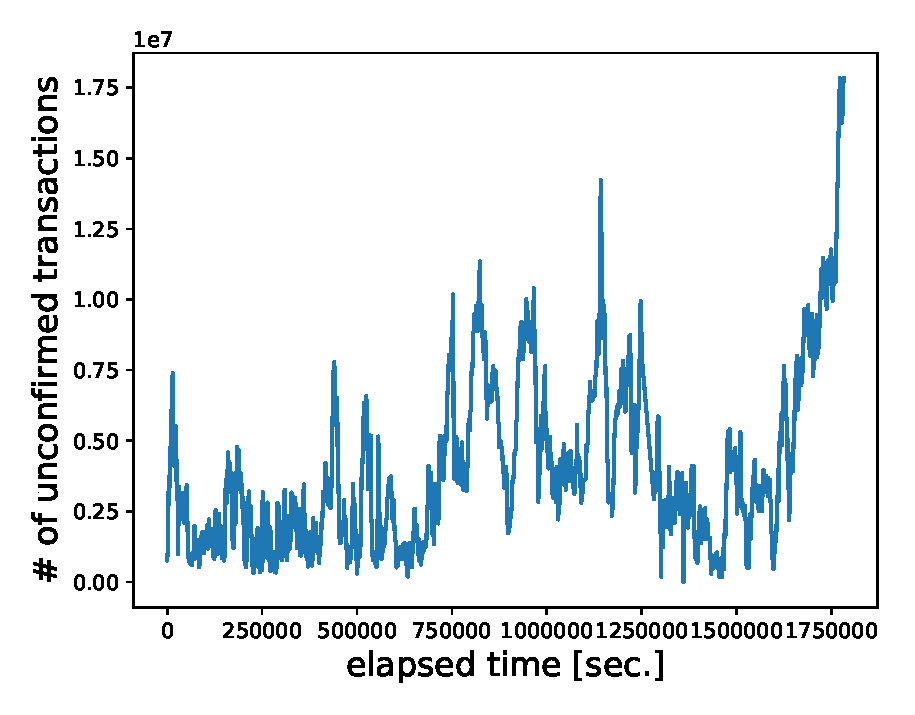
\includegraphics[width=70mm]{time_vs_tx-plot.eps}
  \end{center}
  \vspace{35mm}
  %\caption{STNの未確認取引件数の時間変化}
  \caption{Trend of unconfirmed transactions in STN.}
  \label{fig:unconfirmed_tx}
  %  \ecaption{english caption is here}
\end{figure}
%
We collected the number of unconfirmed transactions periodically from the BSV BC explorer named whatsonchain\cite{woc}.
Figure \ref{fig:unconfirmed_tx} shows that there are regularly more than one million transactions in the transaction pool. 
We can also see that the number of transactions sometimes reaches more than 10 million.


Since STN is open to the public, and anyone can participate in the network. 
However, as system requirements for node construction, the performance of 8--16 cores for CPU, 64 GB (+64 GB Swap) for memory, over 3 TB for hard disk drive, and over 1 Gbit for both up and down Internet connection are required.
The total size of BC was as huge as 2.4 TB at that time in February 9, 2021, while it was only 22 GB in Testnet and 284 GB in Mainnet. 
And, the block height of BC in STN is 15,216 as of February 9, 2021, which is small because BC has been reorganized several times in the past to reduce the BC size. 

CPU mining is possible in STN since the difficulty varies from one to several tens.
The block mining difficulty over time is shown in Fig.~\ref{fig:difficulty}.
%
\begin{figure}[t]
  \vspace{-35mm}
  \begin{center}
    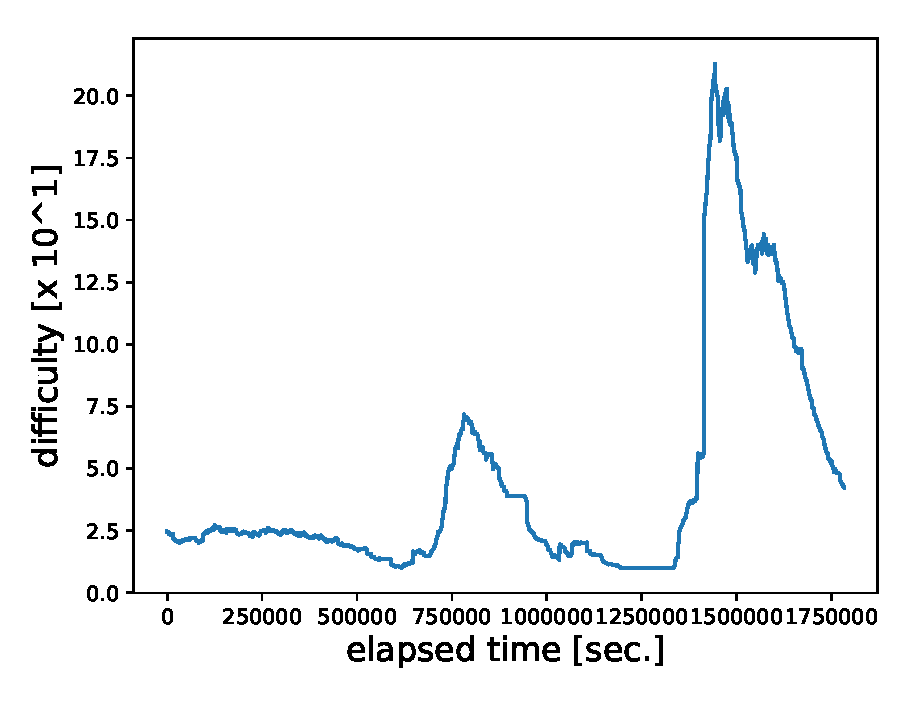
\includegraphics[width=70mm]{time_vs_difficulty-plot.eps}
  \end{center}
  \vspace{35mm}
  %\caption{ブロック採掘の難易度の時間変化}
  \caption{Block mining difficulty over time.}
  \label{fig:difficulty}
  %  \ecaption{english caption is here}
\end{figure}
%

It is recommended that a STN node is configured with a maximum block size of 10 GB and the number of Bitcoin scripts allowable in a transaction is limited to 2GB of memory.
Figures \ref{fig:block_size} show the size distribution of blocks mined so far. 
%
\begin{figure}[t]
  \vspace{-35mm}
  \begin{center}
    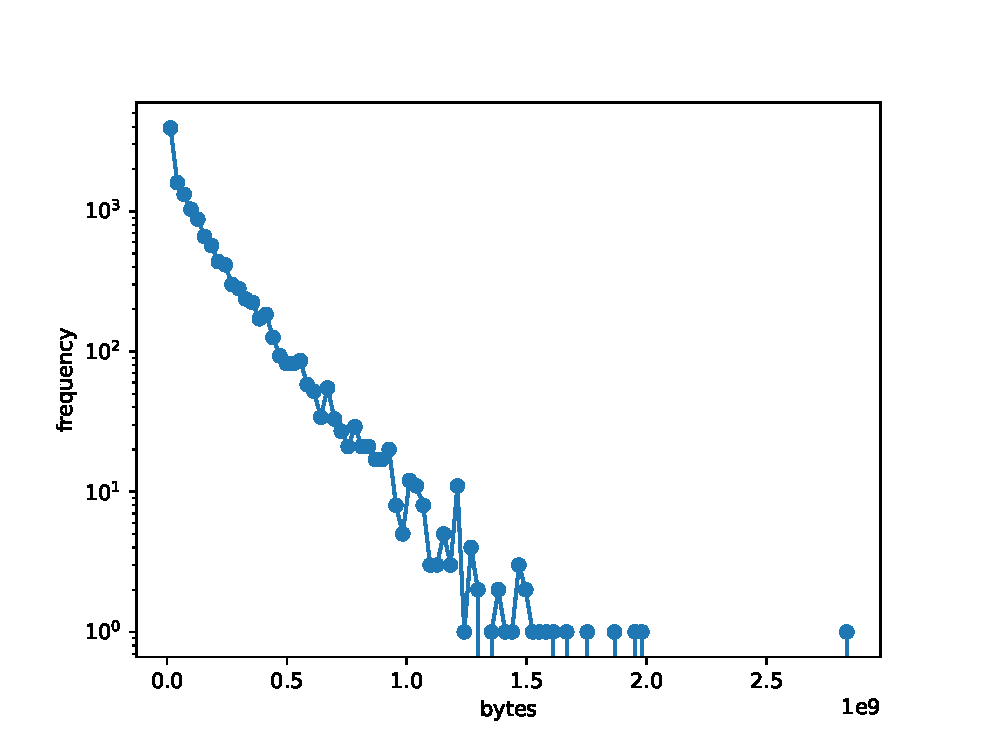
\includegraphics[width=70mm]{bsv_stn-block_bytes-semilogy2.eps}
    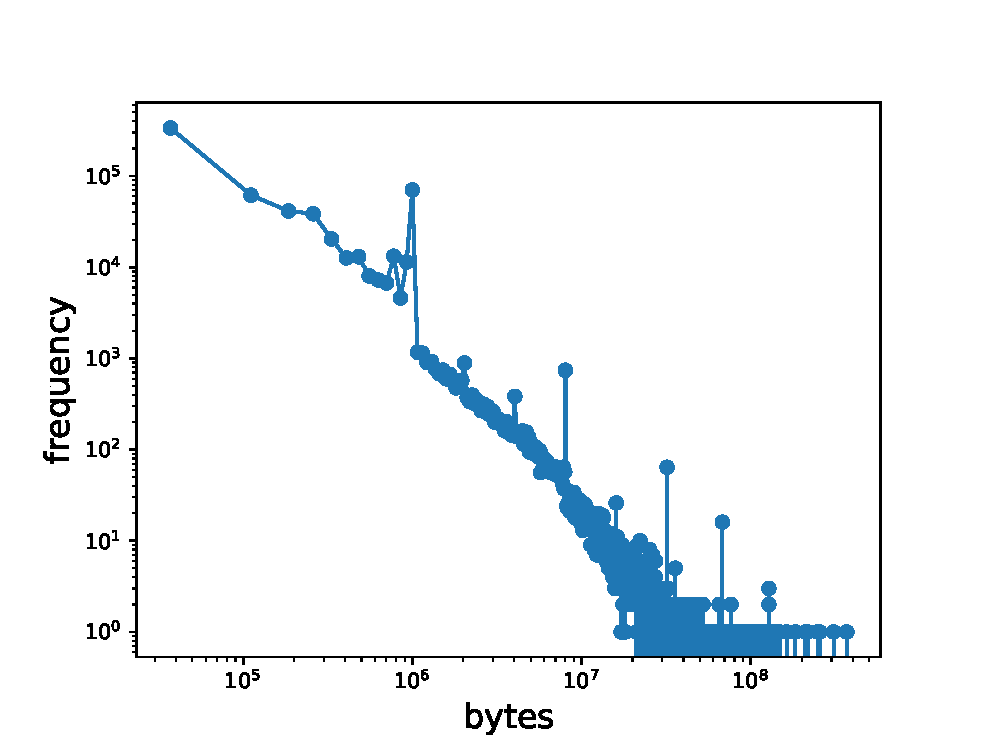
\includegraphics[width=70mm]{bsv_mainnet-block_bytes-loglog.eps}
  \end{center}
  \vspace{35mm}
  \caption{Block size distribution in Bitcoin SV (above is STN, below is Mainnet).}
  \label{fig:block_size}
  %  \ecaption{english caption is here}
\end{figure}
%
The block size distribution of STN seems to follow an exponential distribution.
The largest block size ever mined was 2.9 GB.
On the other hand, the figure below in Figs.~\ref{fig:block_size} shows the block size distribution in Mainnet, which interestingly seems to follow a power-law distribution rather than an exponential distribution.
It also seems to obey the Pareto-Zipf law (= the power-law distribution with its exponent 2). 
This difference in both these distributions might come from the fact that Bitcoin in Mainnet has a market value and that in STN does not, but the reason why they are different is not well understood. 


BSV recommends recording miner ID on mined blocks to assess the reputation of the miners.
Figures \ref{fig:minerrank_stn} and \ref{fig:minerrank_mainnet} show the results of calculating the ranking of block mining frequency with reference to the miner ID.
%
\begin{figure}[t]
  \vspace{-35mm}
  \begin{center}
    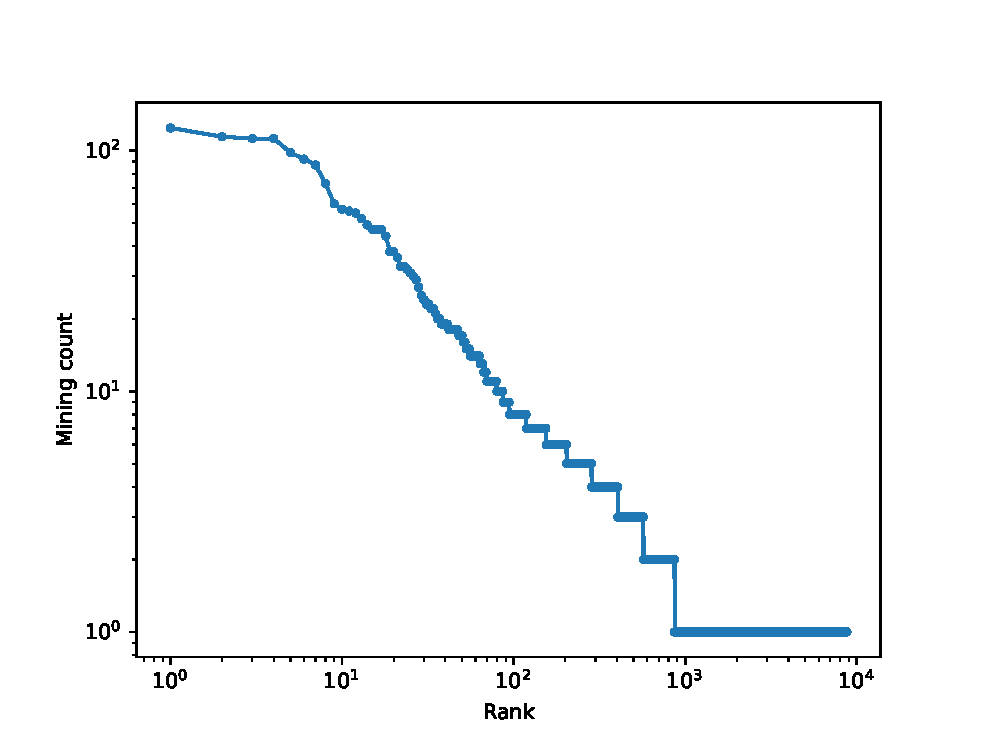
\includegraphics[width=70mm]{bsv_stn-block_miners-ranking-loglog.eps}
  \end{center}
  \vspace{35mm}
  \caption{Block mining frequency ranking calculated with reference to miner ID (STN)}
  \label{fig:minerrank_stn}
  %  \ecaption{english caption is here}
\end{figure}
%
%
\begin{figure}[t]
  %\vspace{-35mm}
  \begin{center}
    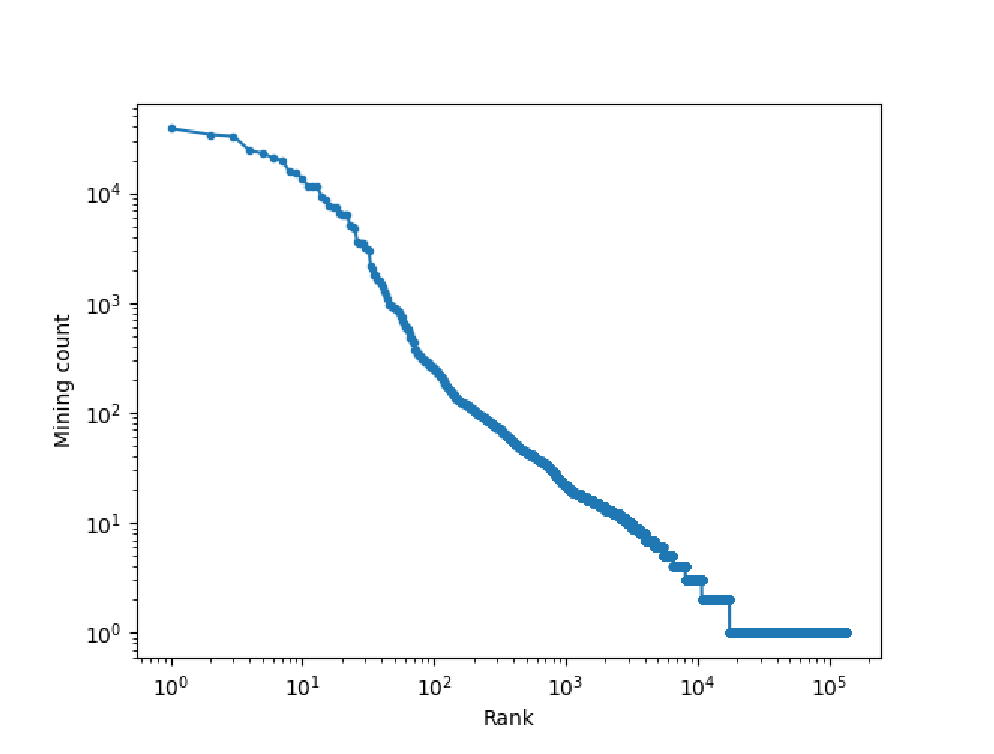
\includegraphics[width=70mm]{bsv_mainnet-block_miners-ranking-loglog.eps}
  \end{center}
  %\vspace{35mm}
  \caption{Block Mining Frequency Ranking Calculated Based on Miner ID (Mainnet)}
  \label{fig:minerrank_mainnet}
  %  \ecaption{english caption is here}
\end{figure}
%
The block mining frequency in both STN and Mainnet seem to follow a power-law distribution.



\section{Performance Evaluation Experiments}
\label{sec:experiments}

\subsection{Experiment 1: Estimating the Occupancy Rate of Approving Transactions in STN}
\label{sec:occupancyrate}

From the time variation of the number of unconfirmed transactions in Fig.~\ref{fig:unconfirmed_tx}, the occupancy rate of STN can be estimated. 
Figure~\ref{fig:occupancyrate} shows the results of calculating the time variation of the estimated occupancy rate of STN $\tilde{\rho}$ based on the queuing theory.
%
\begin{figure}[tb]
  \vspace{-35mm}
  \begin{center}
    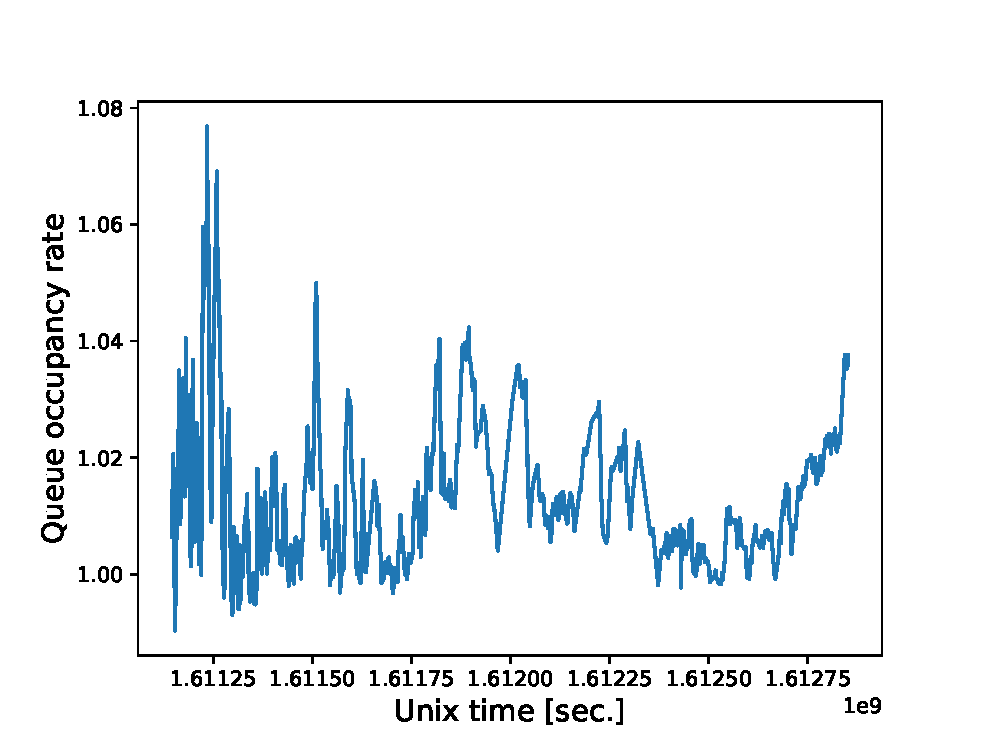
\includegraphics[width=70mm]{bsv_stn-rho-queue_occupancy_rate.eps}
  \end{center}
  \vspace{35mm}
  \caption{Time variation of the estimated occupancy rate in STN $\tilde{\rho}$.}
  \label{fig:occupancyrate}
  %  \ecaption{english caption is here}
\end{figure}
%
 It is observed that the estimated occupancy rate exceeds one in most time period. 
This result suggests that there are almost always unconfirmed transactions. 
Using collected data from November 4, 2020 to February 9, 2021, the estimated occupancy rate was calculated as $\tilde{\rho} \fallingdotseq 1.04$. 
From these results, it is considered that there is a probability of $1 -1 / \tilde{\rho} \fallingdotseq 0.0387$ where transactions are issued but not approved to be finally recorded on BC. 
The reason why transactions are not approved is that STN always have a large number of unconfirmed transactions, but miners tend to approve transactions with higher fees in priority. So, if the fee is low, the transaction approval will be delayed and eventually forgotten because of overflows from the transaction pool. 



\subsection{Experiment 2: Estimating BC Split Probability}
\label{sec:sork}

 If you run an STN node, you will see that when a large block has been generated, a large split of BC will occur and it will go into a safe mode where you will not be able to transfer money using the command \textit{bitcoin-cli}. 
We observed that once this large split of BC occurs, it sometimes takes nearly half a day to resolve.
We conducted an experiment to estimate this BC split probability using warnings when running \textit{bitcoin-cli getinfo}.


During the period from November 4, 2020 to January 13, 2021, warning messages of the command \textit{bitcoin-cli getinfo} were collected once every 10 seconds. We collected them 594,880 times in total. 
Actually, we observed two kinds of warnings as follows.
%
\begin{itemize}
  \item Warning: The network does not appear to fully agree! We received
        headers of a large fork. Still waiting for block data for more details.
	(Occurred 32,724 times, approximately 5.5\% in total.)

  \item Warning: The network does not appear to fully agree! Some miners
        appear to be experiencing issues. A large valid fork has been detected. 
	(Occurred 17,782 times, approximately 3\% in total.)
\end{itemize}
%
From these results, we can estimate the BC split probability to be about $(5.5 + 3 =) 8.5$\%.
This is about four times larger than the BC split probability in BTC. 
By the way, when the split probability of BSV Mainnet was evaluated by the same method, it became 0\%.
If $F(t) = 0.085$ and $\lambda = 1/600$ are substituted in Eq.~(\ref{eq:exp}), then it derives $t = \tau_{fork} \fallingdotseq 53$ seconds, so that the average block propagation time in STN can be estimated to be about 53 seconds. 



\subsection{Experiment 3: Testing Transaction Processing Performance}
\label{sec:method}

In this paper, we experimentally evaluate how long it takes for transactions to be approved in the situation that there are always many transactions in the transaction pool. 
Our experimental period was set for one week from January 7--14, 2021, and the location information of airplanes which flew around Tsudanuma city where Chiba Institute of Technology is located was collected using ADS-B \cite{flightradar24} every one minutes. 
To do this, we wrote a node program to automatically generate transactions including the collected data using OP\_RETURN script to send the P2P network. 
In the experimental settings, the data size per transaction was less than 63 KB and the transaction fee was fixed at 0.001 BSV. 
Additional details about the results are available on our Github website 
\footnote{\url{https://github.com/cit-fujihalab/stn_experiments}}.


Figure~\ref{fig:exp3-1} shows the relation between the elapsed time of the experiment period and the block number where the transaction was approved. 
%
\begin{figure}[tb]
  %\vspace{-35mm}
  \begin{center}
    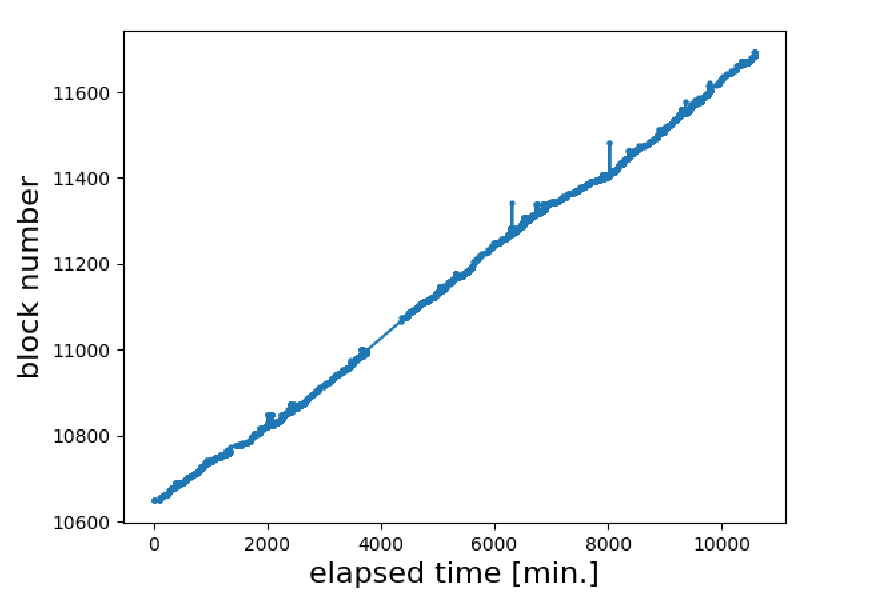
\includegraphics[width=70mm]{exp3-1.eps}
  \end{center}
  %\vspace{35mm}
  \caption{Relation between the elapsed time and the block number where the transaction was approved.}
  \label{fig:exp3-1}
  %  \ecaption{english caption is here}
\end{figure}
%
In total 6,828 transactions were sent during the experimental period, and 104 of them were not recorded in BC. 
From this, the probability that the transaction is not approved can be calculated as $(104/6828 \fallingdotseq) 0.02$.
This result is almost the same as the result calculated in Fig.~\ref{sec:occupancyrate}. 


A histogram of the latency time of the transaction to be approved is shown in Fig.~\ref{fig:exp3-2}.
%
\begin{figure}[t]
  %\vspace{-35mm}
  \begin{center}
    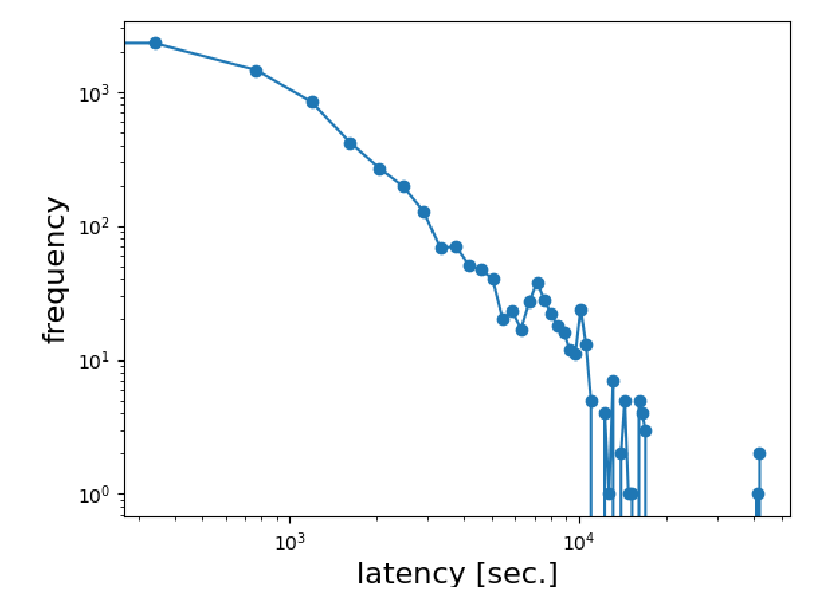
\includegraphics[width=70mm]{exp3-2.eps}
  \end{center}
  %\vspace{35mm}
  \caption{Histogram of latency time of transaction to be approved.}
  \label{fig:exp3-2}
  %  \ecaption{english caption is here}
\end{figure}
%
Since the distribution of block generation time interval follows the exponential distribution, the latency time also follows the exponential distribution in the short term which are about half a day, but it deviates from the exponential distribution in the long term which are about one week.
As shown in Fig.~\ref{fig:exp3-2}, a linear trend appears in the double-logarithmic plot, which indicates the power-law distribution.
The power-law exponent can be estimated from the slope of the double-logarithm plot and is close to 3/2.
These results are consistent with the theoretical analysis of priority queueing.
This indicates that the transaction with low fee becomes low priority, and it takes more time to be finally approved than that with high fee. 


Figure \ref{fig:exp3-3} shows the relation between the fee rate, which is the ratio of transaction fee per byte of transaction, and the latency time until the transaction is approved. 
%
\begin{figure}[t]
  %\vspace{-35mm}
  \begin{center}
    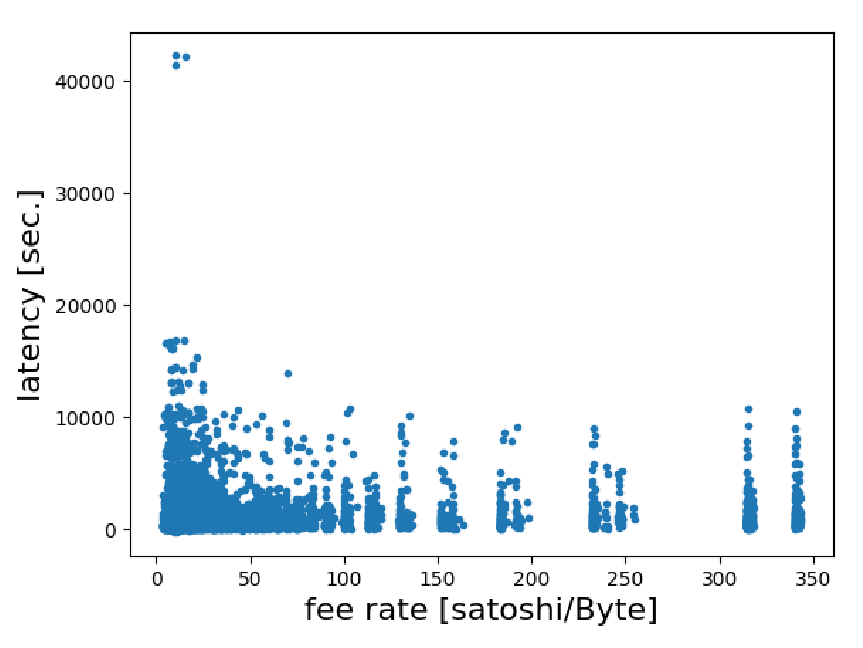
\includegraphics[width=70mm]{exp3-3.eps}
  \end{center}
  %\vspace{35mm}
  \caption{Relation between the fee rate and the latency time until the transaction is approved.}
  \label{fig:exp3-3}
  %  \ecaption{english caption is here}
\end{figure}
%
A low fee rate indicates that it is taking a long time for transactions to be finally recorded on BC.
From the results above, we conclude that it is consistent to analyze STN using the theory of priority queueing as well as BTC. 



\section{Conclusion}
\label{sec:conclusion}

In this study, we conducted data analysis and performance evaluation of Bitcoin SV STN where the upper block size limit is removed. 
As a result of examining the time variation of the occupancy rate of transaction processing capacity, we showed that the estimated occupancy rate almost always exceeded one. 
Using the command \textit{bitcoin-cli getinfo}, we estimated the BC split probability. 
We showed that the probaiblity for STN is about 8.5\%, which is more than 4 times larger than that for BTC.
The average block propagation time of the P2P network was also estimated as about 53 seconds.
The performance of transaction processing was also experimentally evaluated by sending transactions including flight data with OP\_RETURN scripts once per minute during one week.
As a result, it was found that the probability of transactions being approved was 98\%, and the latency time follows the power-law distribution in the long term. 
We also confirmed that the power-law exponent is about 3/2, which is consistent with the theory of priority queueing.
From these results, we concluded that it is consistent to analyze STN using the theory with priority queueing as well as BTC. 



\begin{acknowledgement}
 This work was partially supported by the Japan Society for the Promotion of 
Science (JSPS) through KAKENHI (Grants-in-Aid for Scientific Research) Grant 
Number 20K11797. 
\end{acknowledgement}



%%
%\section*{Appendix}
%\addcontentsline{toc}{section}{Appendix}
%%
%%




\begin{thebibliography}{99}

% Blockchain
\bibitem{HS1991}
  S. Haber and W. S. Stornetta, 
  ``How To Time-Stamp a Digital Document,''
  J. Cryptology, 3, 99-111 (1991)
  %\url{https://link.springer.com/content/pdf/10.1007\%2FBF00196791.pdf}

\bibitem{BHS1993}
  D. Bayer, S. Haber, and W. S. Stornetta,
  ``Improving the Efficiency and Reliability of Digital Time-Stamping,''
  Sequences II: Methods in Communication, Security, and Computer Science, 
  pp. 329-334 (1993).

\bibitem{HS1997}
  S. Haber and W. S. Stornetta, 
  ``Secure Names for Bit-Strings,''
  CCS'97: Proceedings of the 4th ACM conference on Computer and 
  communications security, pp. 28-35 (1997).
  %\url{https://nakamotoinstitute.org/static/docs/secure-names-bit-strings.pdf}


% Bitcoin
\bibitem{nakamoto}
  S. Nakamoto, 
  ``Bitcoin: A Peer-to-Peer Electronic Cash System''
  (White paper), 2008 
  \url{https://bitcoin.org/bitcoin.pdf}
  \url{https://www.bitcoinsv.io/bitcoin.pdf}


% Proof of Work
\bibitem{DN1993}
  C. Dwork and M. Naor, 
  ``Pricing via Processing or Combating Junk Mail,''
  Advances in Cryptology (CRYPTO'92), 
  Lecture Notes in Computer Science, vol. 740, Springer (1993). 
  %\url{https://web.cs.dal.ca/~abrodsky/7301/readings/DwNa93.pdf}


\bibitem{JJ1999}
  M. Jakobsson and A. Juels, 
  ``Proofs of Work and Bread Pudding Protocols (Extended Abstract),''
  In: Preneel B. (eds) Secure Information Networks, 
  The International Federation for Information Processing, 
  vol 23, Springer (1999).
  %\url{https://www.arijuels.com/wp-content/uploads/2013/09/PoW.pdf}


\bibitem{btc}
  Bitcoin Core 
  \url{https://github.com/bitcoin/bitcoin}


% scalability problem
\bibitem{ZHZB2020}
  Q. Zhou, \textit{et al.}, 
  ``Solutions to Scalability of Blockchain: A Survey''
  IEEE Access, Vol. 8, pp.16440-16455, IEEE, 2020. 


\bibitem{Fujihara2018}
  A. Fujihara,
  ``Proposing a System for Collaborative Traffic Information Gathering and 
  Sharing Incentivized by Blockchain Technology,''
  The 10th International Conference on Intelligent Networking and 
  Collaborative Systems (INCoS-2018), pp.170-182 (2018)
  \url{https://link.springer.com/chapter/10.1007/978-3-319-98557-2_16}

\bibitem{Fujihara2019}
  A. Fujihara,
  ``PoWaP: Proof of Work at Proximity for a crowdsensing system for 
  collaborative traffic information gathering,'' 
  Internet of Things, 100046, Elsevier (2019).
  \url{https://www.sciencedirect.com/science/article/pii/S254266051830177X}

\bibitem{Fujihara2020}
  A. Fujihara, 
  ``Proposing a Blockchain-Based Open Data Platform and Its Decentralized Oracle,''
  Advances in Intelligent Networking and Collaborative Systems (INCoS2019), 
  Advances in Intelligent Systems and Computing, 
  Vol. 1035, pp. 190--201, Springer (2020).
  \url{https://link.springer.com/chapter/10.1007/978-3-030-29035-1_19}

\bibitem{YF2021a}
  T. Yanagihara and A. Fujihara, 
  ``Considering Cross-Referencing Method for Scalable Public Blockchain,''
  Advances in Internet, Data and Web Technologies, 
  Lecture Notes on Data Engineering and Communications Technologies, 
  Vol. 65, pp. 220-231, Springer (2021). 
  \url{https://link.springer.com/chapter/10.1007/978-3-030-70639-5_21}

\bibitem{YF2021b}
  T. Yanagihara and A. Fujihara,
  ``Cross-Referencing Method for Scalable Public Blockchain,''
  Internet of Things, Vol. 15, 100419 (2021). 
  \url{https://www.sciencedirect.com/science/article/pii/S2542660521000639}


\bibitem{PD2016}
  J. Poon and T. Dryja, 
  ``The Bitcoin Lightning Network: Scalable Off-Chain Instant Payments,'' 
  (2016) \url{https://lightning.network/lightning-network-paper.pdf}


\bibitem{silkroad}
  FBI, 
  ``Manhattan U.S. Attorney Announces Seizure of Additional \$28 Million 
    Worth of Bitcoins Belonging to Ross William Ulbricht, Alleged Owner 
    and Operator of ``Silk Road'' Website, '' 2013.
%  \url{https://archives.fbi.gov/archives/newyork/press-releases/2013/manhattan-u.s.-attorney-announces-seizure-of-additional-28-million-worth-of}\\
%  \url{-bitcoins-belonging-to-ross-william-ulbricht-alleged-owner-and}\\
%  \url{-operator-of-silk-road-website}

\bibitem{alphabay}
  The US Department of Justice,
  ``AlphaBay, the Largest Online 'Dark Market,' Shut Down,'' 2017.
%  \url{https://www.justice.gov/opa/pr/alphabay-largest-online-dark-market-shut-down}

\bibitem{welcome2video}
  The US Department of Justice,
  ``South Korean National and Hundreds of Others Charged Worldwide in the Takedown 
    of the Largest Darknet Child Pornography Website, Which was Funded by Bitcoin,'' 
  2019.
%  \url{https://www.justice.gov/opa/pr/south-korean-national-and-hundreds-others-charged-worldwide}\\
%  \url{-takedown-largest-darknet-child}



\bibitem{bloX}
  U. Klarman, \textit{et al.},
  ``bloXroute: A Scalable Trustless Blockchain Distribution Network''
  (White paper), 2018.
  \url{https://bloxroute.com/wp-content/uploads/2018/03/bloXroute-whitepaper.pdf}


\bibitem{bsv}
  Bitcoin SV (Satoshi Vision) 
  \url{https://github.com/bitcoin-sv/bitcoin-sv}

\bibitem{bitcoinscaling}
  Bitcoin Scaling Test Network
  \url{https://bitcoinscaling.io/}




\bibitem{OB2005}
  J. G. Oliveira and A.-L. Barab\'asi,
  ``Darwin and Einstein correspondence patterns,'' 
  Nature 437, 1251, 2005.


\bibitem{KK2019}
  S. Kasahara and J. Kawahara,
  ``Effect of Bitcoin fee on transaction-confirmation process,''
  Journal of Industrial and Management Optimization, 15 (1): 365-386, 2019.


\bibitem{woc}
  WhatsOnChain.com, BSV Explorer - STN,
  \url{https://stn.whatsonchain.com/}



% Flightradar24
\bibitem{flightradar24}
  Flight Tracker | Flightradar24 | Track Planes in Real-time,
  \url{https://www.flightradar24.com/}



\end{thebibliography}

\end{document}
